%  LaTeX support: latex@mdpi.com 
%  For support, please attach all files needed for compiling as well as the log file, and specify your operating system, LaTeX version, and LaTeX editor.

%=================================================================
\documentclass[journal,article,submit,pdftex,moreauthors]{Definitions/mdpi} 
\usepackage{caption}
\usepackage[utf8]{inputenc}
%--------------------
% Class Options:
%--------------------
%----------
% journal
%----------
% Choose between the following MDPI journals:
% acoustics, actuators, addictions, admsci, adolescents, aerobiology, aerospace, agriculture, agriengineering, agrochemicals, agronomy, ai, air, algorithms, allergies, alloys, analytica, analytics, anatomia, animals, antibiotics, antibodies, antioxidants, applbiosci, appliedchem, appliedmath, applmech, applmicrobiol, applnano, applsci, aquacj, architecture, arm, arthropoda, arts, asc, asi, astronomy, atmosphere, atoms, audiolres, automation, axioms, bacteria, batteries, bdcc, behavsci, beverages, biochem, bioengineering, biologics, biology, biomass, biomechanics, biomed, biomedicines, biomedinformatics, biomimetics, biomolecules, biophysica, biosensors, biotech, birds, bloods, blsf, brainsci, breath, buildings, businesses, cancers, carbon, cardiogenetics, catalysts, cells, ceramics, challenges, chemengineering, chemistry, chemosensors, chemproc, children, chips, cimb, civileng, cleantechnol, climate, clinpract, clockssleep, cmd, coasts, coatings, colloids, colorants, commodities, compounds, computation, computers, condensedmatter, conservation, constrmater, cosmetics, covid, crops, cryptography, crystals, csmf, ctn, curroncol, cyber, dairy, data, ddc, dentistry, dermato, dermatopathology, designs, devices, diabetology, diagnostics, dietetics, digital, disabilities, diseases, diversity, dna, drones, dynamics, earth, ebj, ecologies, econometrics, economies, education, ejihpe, electricity, electrochem, electronicmat, electronics, encyclopedia, endocrines, energies, eng, engproc, entomology, entropy, environments, environsciproc, epidemiologia, epigenomes, est, fermentation, fibers, fintech, fire, fishes, fluids, foods, forecasting, forensicsci, forests, foundations, fractalfract, fuels, future, futureinternet, futurepharmacol, futurephys, futuretransp, galaxies, games, gases, gastroent, gastrointestdisord, gels, genealogy, genes, geographies, geohazards, geomatics, geosciences, geotechnics, geriatrics, grasses, gucdd, hazardousmatters, healthcare, hearts, hemato, hematolrep, heritage, higheredu, highthroughput, histories, horticulturae, hospitals, humanities, humans, hydrobiology, hydrogen, hydrology, hygiene, idr, ijerph, ijfs, ijgi, ijms, ijns, ijpb, ijtm, ijtpp, ime, immuno, informatics, information, infrastructures, inorganics, insects, instruments, inventions, iot, j, jal, jcdd, jcm, jcp, jcs, jcto, jdb, jeta, jfb, jfmk, jimaging, jintelligence, jlpea, jmmp, jmp, jmse, jne, jnt, jof, joitmc, jor, journalmedia, jox, jpm, jrfm, jsan, jtaer, jvd, jzbg, kidneydial, kinasesphosphatases, knowledge, land, languages, laws, life, liquids, literature, livers, logics, logistics, lubricants, lymphatics, machines, macromol, magnetism, magnetochemistry, make, marinedrugs, materials, materproc, mathematics, mca, measurements, medicina, medicines, medsci, membranes, merits, metabolites, metals, meteorology, methane, metrology, micro, microarrays, microbiolres, micromachines, microorganisms, microplastics, minerals, mining, modelling, molbank, molecules, mps, msf, mti, muscles, nanoenergyadv, nanomanufacturing,\gdef\@continuouspages{yes}} nanomaterials, ncrna, ndt, network, neuroglia, neurolint, neurosci, nitrogen, notspecified, %%nri, nursrep, nutraceuticals, nutrients, obesities, oceans, ohbm, onco, %oncopathology, optics, oral, organics, organoids, osteology, oxygen, parasites, parasitologia, particles, pathogens, pathophysiology, pediatrrep, pharmaceuticals, pharmaceutics, pharmacoepidemiology,\gdef\@ISSN{2813-0618}\gdef\@continuous pharmacy, philosophies, photochem, photonics, phycology, physchem, physics, physiologia, plants, plasma, platforms, pollutants, polymers, polysaccharides, poultry, powders, preprints, proceedings, processes, prosthesis, proteomes, psf, psych, psychiatryint, psychoactives, publications, quantumrep, quaternary, qubs, radiation, reactions, receptors, recycling, regeneration, religions, remotesensing, reports, reprodmed, resources, rheumato, risks, robotics, ruminants, safety, sci, scipharm, sclerosis, seeds, sensors, separations, sexes, signals, sinusitis, skins, smartcities, sna, societies, socsci, software, soilsystems, solar, solids, spectroscj, sports, standards, stats, std, stresses, surfaces, surgeries, suschem, sustainability, symmetry, synbio, systems, targets, taxonomy, technologies, telecom, test, textiles, thalassrep, thermo, tomography, tourismhosp, toxics, toxins, transplantology, transportation, traumacare, traumas, tropicalmed, universe, urbansci, uro, vaccines, vehicles, venereology, vetsci, vibration, virtualworlds, viruses, vision, waste, water, wem, wevj, wind, women, world, youth, zoonoticdis 
% For posting an early version of this manuscript as a preprint, you may use "preprints" as the journal. Changing "submit" to "accept" before posting will remove line numbers.

%---------
% article
%---------
% The default type of manuscript is "article", but can be replaced by: 
% abstract, addendum, article, book, bookreview, briefreport, casereport, comment, commentary, communication, conferenceproceedings, correction, conferencereport, entry, expressionofconcern, extendedabstract, datadescriptor, editorial, essay, erratum, hypothesis, interestingimage, obituary, opinion, projectreport, reply, retraction, review, perspective, protocol, shortnote, studyprotocol, systematicreview, supfile, technicalnote, viewpoint, guidelines, registeredreport, tutorial
% supfile = supplementary materials

%----------
% submit
%----------
% The class option "submit" will be changed to "accept" by the Editorial Office when the paper is accepted. This will only make changes to the frontpage (e.g., the logo of the journal will get visible), the headings, and the copyright information. Also, line numbering will be removed. Journal info and pagination for accepted papers will also be assigned by the Editorial Office.

%------------------
% moreauthors
%------------------
% If there is only one author the class option oneauthor should be used. Otherwise use the class option moreauthors.

%---------
% pdftex
%---------
% The option pdftex is for use with pdfLaTeX. Remove "pdftex" for (1) compiling with LaTeX & dvi2pdf (if eps figures are used) or for (2) compiling with XeLaTeX.

%=================================================================
% MDPI internal commands - do not modify
\firstpage{1} 
\makeatletter 
\setcounter{page}{\@firstpage} 
\makeatother
\pubvolume{1}
\issuenum{1}
\articlenumber{0}
\pubyear{2023}
\copyrightyear{2023}
%\externaleditor{Academic Editor: Firstname Lastname}
\datereceived{ } 
\daterevised{ } % Comment out if no revised date
\dateaccepted{ } 
\datepublished{ } 
%\datecorrected{} % For corrected papers: "Corrected: XXX" date in the original paper.
%\dateretracted{} % For corrected papers: "Retracted: XXX" date in the original paper.
\hreflink{https://doi.org/} % If needed use \linebreak
%\doinum{}
%\pdfoutput=1 % Uncommented for upload to arXiv.org

%=================================================================
% Add packages and commands here. The following packages are loaded in our class file: fontenc, inputenc, calc, indentfirst, fancyhdr, graphicx, epstopdf, lastpage, ifthen, float, amsmath, amssymb, lineno, setspace, enumitem, mathpazo, booktabs, titlesec, etoolbox, tabto, xcolor, colortbl, soul, multirow, microtype, tikz, totcount, changepage, attrib, upgreek, array, tabularx, pbox, ragged2e, tocloft, marginnote, marginfix, enotez, amsthm, natbib, hyperref, cleveref, scrextend, url, geometry, newfloat, caption, draftwatermark, seqsplit
% cleveref: load \crefname definitions after \begin{document}

%=================================================================
% Please use the following mathematics environments: Theorem, Lemma, Corollary, Proposition, Characterization, Property, Problem, Example, ExamplesandDefinitions, Hypothesis, Remark, Definition, Notation, Assumption
%% For proofs, please use the proof environment (the amsthm package is loaded by the MDPI class).

%=================================================================
% Full title of the paper (Capitalized)
\Title{Numerical study of an influence of pulsed laser deposited TiN
thin films microstructure morphologies on strain heterogenei-
ties during mechanical testing}

% MDPI internal command: Title for citation in the left column
\TitleCitation{Title}

% Author Orchid ID: enter ID or remove command
\newcommand{\orcidauthorA}{0000-0000-0000-000X} % Add \orcidA{} behind the author's name
%\newcommand{\orcidauthorB}{0000-0000-0000-000X} % Add \orcidB{} behind the author's name

% Authors, for the paper (add full first names)
\Author{Konrad Perzynski $^{1}$, Grzegorz Cios $^{2}$, Grzegorz Szwachta $^{2}$, Piotr Bała$^{1,2}$ and Lukasz Madej$^{1}$}

%\longauthorlist{yes}

% MDPI internal command: Authors, for metadata in PDF
\AuthorNames{Konrad Perzynski, Grzegorz Cios,Grzegorz Szwachta,Piotr Bała and Lukasz Madej}

% MDPI internal command: Authors, for citation in the left column
\AuthorCitation{Lastname, F.; Lastname, F.; Lastname, F.}
% If this is a Chicago style journal: Lastname, Firstname, Firstname Lastname, and Firstname Lastname.

% Affiliations / Addresses (Add [1] after \address if there is only one affiliation.)
\address{%
$^{1}$ \quad Faculty of Metals Engineering and Industrial Computer Science, AGH University of Science and Technology, Mickiewicza 30 av., 30-059 Krakow, Poland; kperzyns@agh.edu.pl\\
$^{2}$ \quad Academic Centre for Materials and Nanotechnology, AGH University of Science and Technology, Mickiewicza 30 av., 30-059 Krakow, Poland; grzegorz.cios@agh.edu.pl}

% Contact information of the corresponding author
\corres{Correspondence: kperzyns@agh.edu.pl; Tel.:+48-12-617-50-08}

% Current address and/or shared authorship
%\firstnote{Current address: Affiliation 3.} 
%\secondnote{These authors contributed equally to this work.}
% The commands \thirdnote{} till \eighthnote{} are available for further notes

%\simplesumm{} % Simple summary

%\conference{} % An extended version of a conference paper

% Abstract (Do not insert blank lines, i.e. \\) 
\abstract{Influence of pulsed laser deposited TiN thin films microstructure morphologies on strain heterogeneities during loading was the goal of this research. The investigation was based on the digital material representation concept applied to replicate a microstructure morphology of an investigated thin film. The physically-based pulsed laser deposited model was implemented to recreate characteristic features of a thin film microstructure. The kinetic Monte Carlo approach was used as the basis of the model. Obtained results were validated with the experimental data from metallographic analysis of laboratory deposited TiN(100)/Si thin film. Finally, the digital material representation model was incorporated into the multiscale finite element simulation of nanoindentation test to evaluate the development of local deformation heterogeneities associated with the underlying microstructure morphology. In this part, the capabilities of the proposed approach were clearly highlighted.}

% Keywords
\keyword{pulsed laser deposition; thin films; digital material representation; Kinetic Monte Carlo.} 

% The fields PACS, MSC, and JEL may be left empty or commented out if not applicable
%\PACS{J0101}
%\MSC{}
%\JEL{}

%%%%%%%%%%%%%%%%%%%%%%%%%%%%%%%%%%%%%%%%%%
% Only for the journal Diversity
%\LSID{\url{http://}}

%%%%%%%%%%%%%%%%%%%%%%%%%%%%%%%%%%%%%%%%%%
% Only for the journal Applied Sciences
%\featuredapplication{Authors are encouraged to provide a concise description of the specific application or a potential application of the work. This section is not mandatory.}
%%%%%%%%%%%%%%%%%%%%%%%%%%%%%%%%%%%%%%%%%%

%%%%%%%%%%%%%%%%%%%%%%%%%%%%%%%%%%%%%%%%%%
% Only for the journal Data
%\dataset{DOI number or link to the deposited data set if the data set is published separately. If the data set shall be published as a supplement to this paper, this field will be filled by the journal editors. In this case, please submit the data set as a supplement.}
%\datasetlicense{License under which the data set is made available (CC0, CC-BY, CC-BY-SA, CC-BY-NC, etc.)}

%%%%%%%%%%%%%%%%%%%%%%%%%%%%%%%%%%%%%%%%%%
% Only for the journal Toxins
%\keycontribution{The breakthroughs or highlights of the manuscript. Authors can write one or two sentences to describe the most important part of the paper.}

%%%%%%%%%%%%%%%%%%%%%%%%%%%%%%%%%%%%%%%%%%
% Only for the journal Encyclopedia
%\encyclopediadef{For entry manuscripts only: please provide a brief overview of the entry title instead of an abstract.}

%%%%%%%%%%%%%%%%%%%%%%%%%%%%%%%%%%%%%%%%%%
% Only for the journal Advances in Respiratory Medicine
%\addhighlights{yes}
%\renewcommand{\addhighlights}{%

%\noindent This is an obligatory section in “Advances in Respiratory Medicine”, whose goal is to increase the discoverability and readability of the article via search engines and other scholars. Highlights should not be a copy of the abstract, but a simple text allowing the reader to quickly and simplified find out what the article is about and what can be cited from it. Each of these parts should be devoted up to 2~bullet points.\vspace{3pt}\\
%\textbf{What are the main findings?}
% \begin{itemize}[labelsep=2.5mm,topsep=-3pt]
% \item First bullet.
% \item Second bullet.
% \end{itemize}\vspace{3pt}
%\textbf{What is the implication of the main finding?}
% \begin{itemize}[labelsep=2.5mm,topsep=-3pt]
% \item First bullet.
% \item Second bullet.
% \end{itemize}
%}

%%%%%%%%%%%%%%%%%%%%%%%%%%%%%%%%%%%%%%%%%%
\begin{document}
%%%%%%%%%%%%%%%%%%%%%%%%%%%%%%%%%%%%%%%%%%
 
% The order of the section titles is different for some journals. Please refer to the "Instructions for Authors” on the journal homepage.
\section{Introduction}
 
The deposition process of thin films by laser ablation has been known since the '1970's [1]. This method is used in a wide range of industrial applications: from superconductors' production, through the manufacturing of forming tools coatings up to the biocompatible materials for medical implants [2,3].\\
\indent{Deposition} processes are especially interesting in the latter applications as they can provide thin films at the medical equipment and increase both its strength and bio-protection properties [2]. However, in these applications, development of any internal defects in the thin film, due to, e.g., local strain localization occurring during exploitation conditions, is unacceptable. Such defects can cause a build-up of biological material and deterioration of strength properties, which may be hazardous for a patient. That is why morphology of deposited thin layers must ensure all mechanical expectations required for their applications. Presently, there is a wide variety of methods that can be used for deposition purposes. The primary representative of the technologies is the Pulsed Laser Deposition (PLD) method [4], which is a modification of the standard Physical Vapour Deposition (PVD) approach. The main idea of the PLD is based on evaporation and ionization of the surface atoms by a high-power laser beam that is periodically focused on a target. Particles are first detached by a laser and then strike with high speed into the surface of the substrate materials and start to nucleate and grow. This process provides possibilities to obtain layers at different kinds of engineering materials. The stoichiometry of the target material is reflected in the films very well, improving adhesion between the layer and the substrate. These properties result mainly from the fact that particles in an atomic beam have considerable kinetic energies (0.1–100 eV), which increase the diffusion rate of adatoms at the surface [5]. The PLD can be divided into three stages: ablation, transportation of atoms through a chamber and deposition onto a substrate surface. Experimentally, each pulse lasts for a few nanoseconds, and the time between two pulses is of the order of a second. That is why thin layers' growth mechanism by a pulsed laser deposition is an extremely complex process. For this reason, the development of a specific deposition technology for a given material often involves long-term research aimed at an empirical determination of the required process parameters.\\ 
\indent{That} is why, at first, Authors decided to develop a numerical model of the PLD deposition process, which can support experimental research and also provide reliable data on thin film morphologies for further studies of their behaviour under exploitation conditions. Commonly used numerical models of deformation neglect the inner structure of deposited thin films [6,7] what depreciates the quality of obtained data. Deposited material under, e.g., loading conditions is usually defined as isotropic without taking into account columns and surface wrinklings, which are commonly observed under structural investigation. Thus, simplified models cannot give sufficient information about material resistance to deformation. Therefore, the development of the model, which precisely maps thin films' morphologies and inner structures during modelling of exploitation conditions, seems extremely relevant and important to obtain results comparable with those from experimental investigations.\\
\indent{Reliable} digital material representation of thin film microstructure morphology numerical model of the deposition process was developed first. It provides a digital representation model [8,9] of layers for subsequent numerical simulations of deformation under nanoindentation conditions as a function of deposition process parameters. As a result, the complex nanoindentation model will provide a basic understanding of local heterogeneous material response to deformation conditions.
%%%%%%%%%%%%%%%%%%%%%%%%%%%%%%%%%%%%%%%%%%
\section{Numerical modelling of the PLD process}
 
First 2D numerical models of deposition aiming at capturing underlying physics can be found in the literature from early '1970's [10]. Presently, two major types of approaches can be distinguished: the deterministic and the stochastic ones. The most common examples of deterministic models are based on the molecular dynamics method [11–13]. This method describes the movement of individual atoms or material particles by the Newton equation of motion. However, to calculate forces and energies  between atoms, a set of interatomic potentials must be defined. The Molecular Dynamics (MD) method can directly address mechanisms of deposition at the nanoscale. However, due to a small length scale and available computational resources, it only allows investigating a very local material behaviour far beyond the industrial expectations. That is why stochastic models of deposition are more frequently used during the investigation.\\ 
\indent{The} first group of the stochastic methods is based on the Cellular Automata (CA) technique. The CA technique's main idea is to divide a specific part of the material into one-, two-, or three-dimensional lattice of finite cells. Each cell in the CA space is also surrounded by neighbours, which affect one another. The cells interactions within the CA space are based on the knowledge defined while studying a particular phenomenon. An example of the CA's epitaxially thin layers growth simulation was presented in authors earlier works [14–18]. These approaches can be classified as Random Deposition Models (RDM) [19,20] and consist of three main steps: random deposition of particles at the growing surface, calculation of total energy of each particle with the migration of mobile particles along the surface and eventually desorption of particles from the surface.
The second group is based on the Monte Carlo (MC) method. Models, which belong to that group provide a possibility to describe the evolution of complex systems with some simplifications during calculations [21–24]. They are based on a random sampling of the examined quantity with the use of its analytical distributions. However, the MC method does not directly take into account the elapse of time, which is particularly important in the description of systems in which events occur concurrently and are mutually dependent. Because a thin film growth belongs to such systems therefore, a modified version of the MC method was developed to take into account the process kinetics and is called the kinetic Monte Carlo (kMC).\\
\indent{A} group of the kMC methods describes the progression of complex systems by identification of all possible events and assigning to them the probability of occurrence. For that, the method requires knowledge about rates of each event, which are determined based on values of energy barriers that the system has to overcome to move to a new configuration. Statistically, the most likely events are selected more often. The great advantage of the kMC method is a consideration of the physical time of the process during a simulation. With that, it is possible to take into account many competing mechanisms occurring during a deposition process: atoms deposition, diffusion on the surface, island formation, connection/disconnection to/from existing atoms islands, ascending/descending on/from the existing atoms islands and evaporation.\\
\indent{Therefore}, the kMC approach was selected for the current investigation focused on the implementation of the PLD deposition model of TiN thin films.\\
 
\noindent\textbf{Formulation of the kMC PLD deposition model}\\
\indent{To} describe the evolution of the growing layer during the PLD, all mentioned earlier, important processes were grouped into two elementary phenomena:\\
\indent{adsorption} – particles from plasma flux are attached to the substrate surface due to the weak van der Waals forces,\\ 
\indent{surface-diffusion} – particles at the surface can change their sites in favour of energy minimization,\\ 
\indent{A} concept of all mentioned elementary events, which are considered during the kMC model development, is shown in Figure 1.
 
\begin{figure}[h]
  \captionsetup{justification=centering}
  \centering
  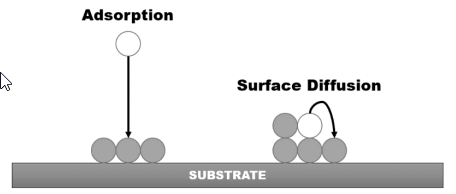
\includegraphics{Definitions/picture1.png}
  \label{fig:obraz1}
    \caption{Elementary events during the PLD accounted for by the developed kMC model.}
    \end{figure}   
\unskip
 
As mentioned, the key information required by the kMC algorithm is related to the rates of these fundamental events, which can be described by the following set of equations:
\begin{itemize}%[label=$\cdot$]
   \item Adsorption rate: \\
  \begin{math}
  r_{ads} = \frac{D}{a}
  \end{math}\\
   where: D – deposition rate, a – dimension of an elementary cell.\\
   \item Surface diffusion rate is given by an Arrhenius-type expression:\\
  \begin{math}
  r_{diff} = \alpha Te^\frac{-\Delta E}{kT}
  \end{math}\\
  where: k – Boltzmann constant, T – relative substrate temperature, $ \alpha$ – adatom \noindent vibration frequency.\\
  Change of an occupied site is driven by an energy difference (activation energy):\\
  \begin{math}
  \Delta E = E_1 - E_0\\
  \end{math}
  where: $E_1$ – energy of a particle after a hypothetic change, $E_0$ – current energy of a particle.\\
  The energy of a given particle is defined as:\\
  \begin{math}
  E=\Sigma_{i}E_i\\
  \end{math}
  where:$E_i$ – binding energy between a considered particle and a particle from a neighbourhood, which is placed at a site $i$.\\
  \indent{The} schematic block diagram of the implemented kMC algorithm is presented in Figure 2.
\end{itemize}\
 
\begin{figure}[h]
    \captionsetup{justification=centering}
    \centering
    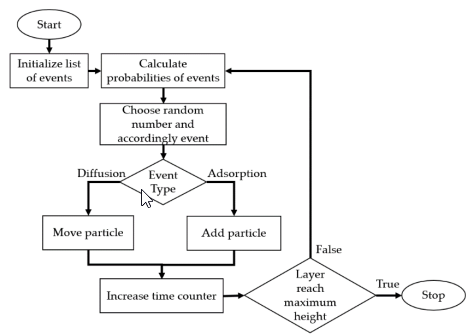
\includegraphics{Definitions/picture2.png}
    \label{fig:obraz2}
    \caption{Block diagram showing the kMC algorithm of the PLD.}
    \end{figure}
 
    Following the kinetic Monte Carlo method for each calculation step, a list of possible events in the system is computed along with probabilities of their occurrence. Then, based on a random number from $\langle 0,R)$, where $R$ is an accumulated probability of all events, a single event is selected and applied to the system.\\
 
Therefore the kMC consists of several steps:
    \begin{enumerate}
        \item Creation of a list of all possible events in the system and calculation of a likelihood of their occurrence $r_i$.
        \item Calculation of the sum of probabilities of all events $R = \Sigma_{j=0}^ir_j$
        \item Random selection of a number in a range $\langle 0,R)$.
        \item Each event is placed on a stack. Graphically (Figure 3), the height of a particular event represents its probability of occurrence. An overall height stack is thus equal to a cumulated probability of all considered events – $R$. A randomly chosen number $\ $ unambiguously indicates the event, which will be applied to the system. Selection of the event is shown in Figure 3.
        \item Transposition of the system to a new state by applying the selected event.
        \item Updating the time counter by $\Delta t = \frac{1}{R}$.
    \end{enumerate}
 
    \begin{figure}[H]
    \captionsetup{justification=centering}
    \centering
    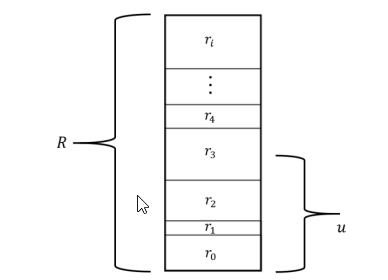
\includegraphics{Definitions/picture3.png}
    \label{fig:obraz3}
    \caption{Method of selecting an event from the available list in the kMC algorithm.}
    \end{figure}
    From the implementation point of view, an aspect that requires particular attention is optimising the algorithm towards reducing computing time. In the classical kMC approach, a list of all events is recreated at each time step, which is a severely CPU time-consuming task. To improve the algorithm’s performance, a list of events can be initialized only once. And later depending on an event, which is selected accordingly up-dated by: 
    \begin{itemize}
        \item adding events, which become possible,
        \item removing obsolete events,
        \item updating probabilities of all events, which could be affected by a previous change in the system.
    \end{itemize}
 
     Keeping track of all events, which will be affected by applying a new event to the system, is challenging. The simplest way to achieve this is to recalculate the probability of directly related events to the extent of the existing neighbourhood. This is because some types of events, i.e. surface diffusion, depend not only on the particles’ actual configuration but also on the configuration after a hypothetical movement of the particle. Example of this procedure is shown in Figure 4. The considered neighbourhood has a radius of a single particle. The red border represents the range of a doubled neighbourhood. Affected particles are thus located in the doubled neighbourhood before and after the particle movement.
    \begin{figure}[H]
    \captionsetup{justification=centering}
    \centering
    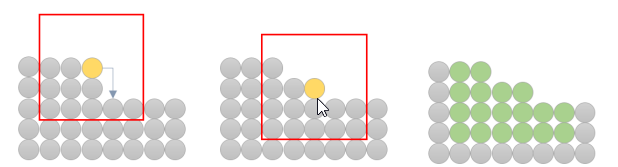
\includegraphics{Definitions/picture4.png}
    \label{fig:obraz3}
    \caption{Procedure of choosing particles, which interrelated events probabilities could be 194
effected (marked as green) after applying a surface  diffusion to the system (marked as 195
yellow).}
    \end{figure}
%%%%%%%%%%%%%%%%%%%%%%%%%%%%%%%%%%%%%%%%%%
\section{Kinetic Monte Carlo simulations of the PLD process}
 
The developed kMC deposition model was used in the work to simulate the growth of the TiN thin film on the single-crystal Si substrate. Deposition process parameters, namely substrate temperature \(T_{sub}\) = 200° C and deposition rate 0.05nm/s were selected to obtain columnar growth. Model parameters presented in Table 1 were selected based on the literature findings [25–27] and a series of initial simulations. 
 
\begin{table}[H] 
\centering
\captionsetup{justification=centering}
\caption{Parameters used in the kMC PLD model of the TiN/Si deposition.\label{tab1}}
\newcolumntype{C}{>{\centering\arraybackslash}X}
\begin{tabularx}{0.7\textwidth}{CC}
\toprule
Parameter	& Value\\
\midrule
Domain edge length &90 nm\\
Elementary cell size &1 nm\\
Substrate melting temperature &1414 ℃\\
Substrate temperature &200 ℃\\
Binding energy	&0.8 eV\\
Deposition rate &0.05 nm/s\\
Vibration frequency &\(1x10^{13}\) Hz\\
\bottomrule
\end{tabularx}
\end{table}
 
The TiN thin film with the dimension of 90nm x 90nm x 90nm was obtained from the kMC simulation. Example of the DMR model of thin film during kMC simulation is shown in Figure 5.
 
\begin{figure}[H]
  \captionsetup{justification=centering}
  \centering
  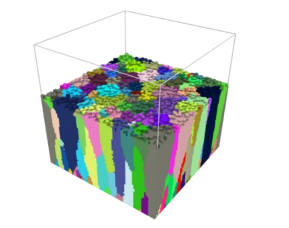
\includegraphics{Definitions/picture5.png}
  \label{fig:obraz5}
    \caption{Microstructure morphology during the kMC simulation of the TiN thin film depo-\\sition.}
\end{figure}   
 
 
As presented in Figure 6, the shape of generated columns in the thin films is highly irregular. Bottom columns are characterized by a lower surface area than the columns in the thin film's upper part. To show a change in columns geometry and the height of the final sample a surface area of each column at subsequent cross-sections (22nm, 45nm, and 67nm) was calculated and presented in Figure 6.
 
\begin{figure}[H]
  \captionsetup{justification=centering}
  \centering
  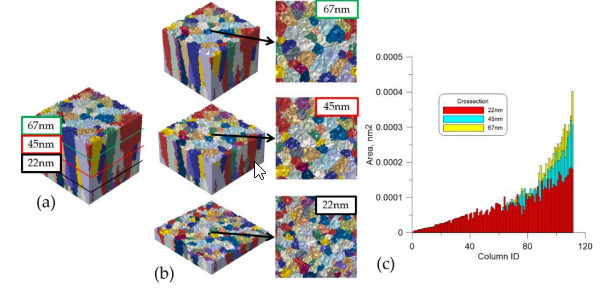
\includegraphics{Definitions/picture6.png}
  \label{fig:obraz6}
    \caption{(a) position of the cross-section in the final DMR sample, (b) illustration of columns at particular cross-sections and (c) diagram representing areas of subsequent columns at particular cross-sections.}
\end{figure}   
 
Additionally, in Figure 7 it can be seen that the average height of the four highest columns is between 87 to 91nm. The average width of those columns in the middle is between 18 to 25nm, but in the top part, an average width increases and is between 19 to 28nm (Figure 6). All columns have a V shape, which can also be observed through the microscopy investigations.
 
\begin{figure}[H]
  \captionsetup{justification=centering}
  \centering
  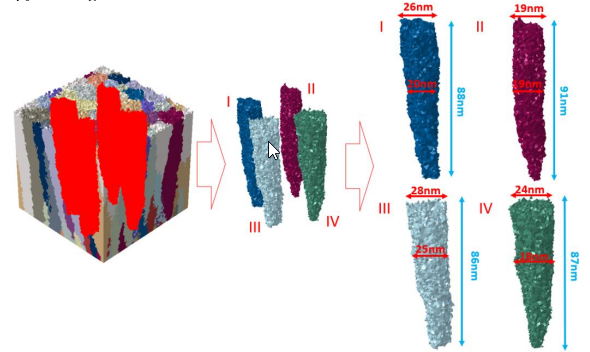
\includegraphics{Definitions/picture7.png}
  \label{fig:obraz7}
    \caption{Dimensions of the columns obtained from PLD simulation.}
\end{figure}   
 
%%%%%%%%%%%%%%%%%%%%%%%%%%%%%%%%%%%%%%%%%%
\section{Experimental investigation}
 
To validate the PLD model predictions, a 90nm TiN thin film was deposited in the laboratory conditions on the Si(100) substrate using the 248nm excimer laser system (Coherent COMPexPro 110F) operated at an energy density of ~3 Jcm-2 , a pulse width of 20ns and a repetition rate of 10 Hz. The target was a disc with 2.54 cm in the diameter and 0.5cm in the thickness. The initial pressure in the chamber was set to 5×10-7 Torr. The silicon substrate was subjected to an ultrasonic cleaning procedure for 10 min in acetone and 10min in methanol and finally etched for 5min in 10\% HF. The substrate was placed parallel to the target material surface at a distance of 5cm. The deposition temperature and nitrogen partial pressure were 200°C and 1×10-5 Torr, respectively [9,28]. Process settings closely replicate the conditions selected during numerical modelling presented earlier.\\ 
\indent{Investigation} of the TiN thin layer morphology was carried out by the transmission electron microscopy (TEM). The sample was prepared for this investigation by a focused ion beam (FIB) technique. The FIB preparation included an electron beam Pt deposition at the beginning and a low accelerating voltage cleaning as the final step. To evaluate deposited columns' thickness, a set of dark field images was taken within the same area using different peak lying on the first ring of the diffraction pattern. Observed columns with marked investigated locations and corresponding dimensions are presented in Figure 8 and Table 2, respectively.
 
\begin{figure}[H]
  \captionsetup{justification=centering}
  \centering
  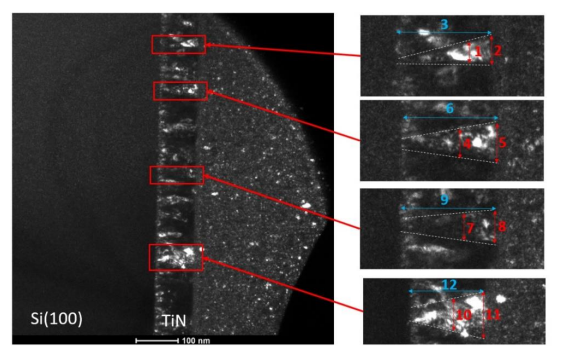
\includegraphics{Definitions/picture8.png}
  \label{fig:obraz8}
    \caption{TEM images with marked investigated locations}
\end{figure}   
 
\begin{table}[H] 
{\caption{Measured columns dimensions in the TiN thin film ({\color{red}{width}}, {\color{cyan}{high}}).\label{tab2}}
\newcolumntype{C}{>{\centering\arraybackslash}X}
\begin{tabularx}{\textwidth}{lCCCCCCCCCCCC}
\toprule
dimension number &{\color{red}{1}}    &{\color{red}{2}}    &{\color{cyan}{3}}    &{\color{red}{4}}    &{\color{red}{5}}    &{\color{cyan}{6}}    &{\color{red}{7}}    &{\color{red}{8}}    &{\color{cyan}{9}}    &{\color{red}{10}}   &{\color{red}{11}} &{\color{cyan}{12}}   \\
\midrule
size [nm]    &{\color{red}{15.1}} &{\color{red}{25.9}} &{\color{cyan}{89.1}} &{\color{red}{24.8}} &{\color{red}{33.1}} &{\color{cyan}{94.4}} &{\color{red}{23.6}} &{\color{red}{30.5}} &{\color{cyan}{87.6}} &{\color{red}{30.8}} &{\color{red}{53}} &{\color{cyan}{93.6}}\\
\bottomrule
\end{tabularx}
\end{table}
 
As seen in Figure 7, Figure 8 and Table 2, the numerical model predictions appropriately replicate experimental observations. Therefore, the developed PLD model can be used to generate realistic morphologies of thin films for further numerical investigations of their behaviour under, e.g., loading conditions based on the mentioned digital material representation concept. 
 
%%%%%%%%%%%%%%%%%%%%%%%%%%%%%%%%%%%%%%%%%%
\section{Numerical nanoindentation test based on the explicit representation of thin films morphologies.}
 
The nanoindentation test, which is commonly used to evaluate thin films' mechanical properties, was selected as a case study for the present investigation. The partially coupled concurrent multiscale methodology was used due to a significant length scale difference between the microscopic model of the nanoindentation test and nanoscale model based on the digital material representation. In this approach, a particular area of interest from the macro scale model is selected and recalculated with a refined mesh to obtain a more detailed solution. The microscale model contains information on the sample geometry and boundary conditions of the nanoindentation test. Additional features related to the nanoscale model, e.g. columnar morphology, are initially excluded at this length scale. On the other hand, the nanoscale model is an arbitrary cut–out taken from the micromodel and it takes into account the digital model of the thin film morphology obtained from the develop kMC algorithm. In this procedure, the microscale model is first calculated within the Abaqus/Explicit. The refined nanoscale model is resubmitted for simulation with displacement boundary conditions taken from the micro model simulation. A schematic description of this multiscale technique applied for the nanoindentation test is presented in Figure 9.
 
\begin{figure}[H]
  \captionsetup{justification=centering}
  \centering
  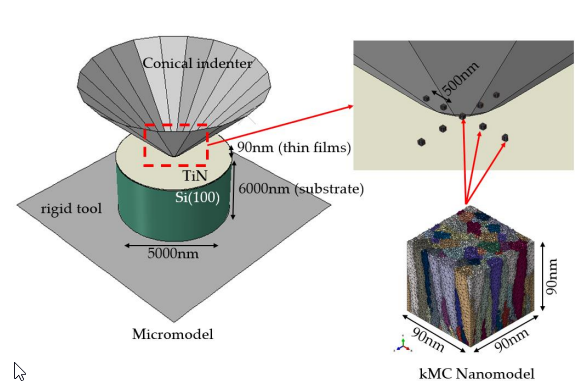
\includegraphics[width=\linewidth]{Definitions/picture9.png}
  \label{fig:obraz9}
    \caption{Schematic illustration of the multi scale model of the nanoindentation test.}
\end{figure}  
 
During the simulation, a diamond nanoindenter is assumed to be a deformable body with elastic modulus and 'Poisson's ratio taken from the literature [29]. The micro model of the thin film was discretized with 150000 8-node tetrahedron elements. Additionally, a displacement of the Si(100) substrate was fixed by the rigid tool situated at the bottom of the sample.\\
\indent{Examples} of results obtained from the micromodel are shown in Figure 10. As mentioned, they are then used as boundary conditions for the nanoscale model, which include a columnar morphology of the thin film.
 
\begin{figure}[H]
  \captionsetup{justification=centering}
  \centering
  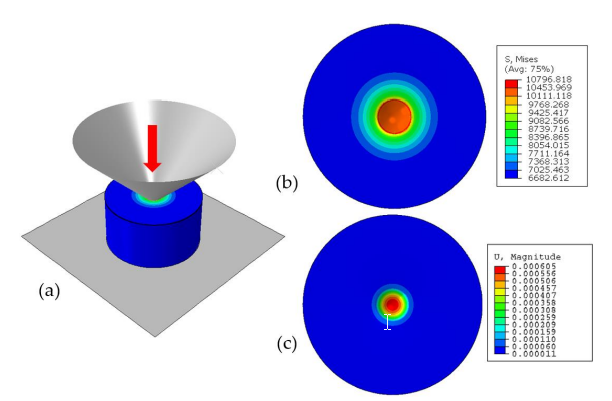
\includegraphics[width=\linewidth]{Definitions/picture10.png}
  \label{fig:obraz10}
    \caption{Distribution of \textbf{(a)} equivalent stress (MPa) in the model from the side view and, \\\textbf{(b)} equivalent stress (MPa), \textbf{(c)} displacement (mm) from the top view.}
\end{figure}  
 
As mentioned, the nanoscale model is based on the thin film morphology presented in Figure 7. The possibility of assigning material properties to particular TiN columns was described in the previous work [28]. The generated morphology was also subjected to a discretization algorithm. The non-uniform mesh was created using a DMRmesh software [30]. The FE mesh (Figure 11) is highly refined along the columns' boundaries to adequately capture solution gradients that are expected in these regions due to differences in hardening behaviour of subsequent columns. 
 
\begin{figure}[H]
  \captionsetup{justification=centering}
  \centering
  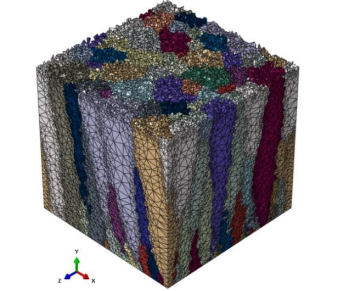
\includegraphics{Definitions/picture11.png}
  \label{fig:obraz11}
    \caption{Finite element mesh of the investigated TiN thin film columnar morphology.}
\end{figure}  
 
The thin film DMR model was discretized with 631000 four-node linear tetrahedron (C3D4) elements (Figure 11). Such nanoscale model was then located in 9 different location within the deformation area, according to Figure 9. Examples of results presenting the influence of a columnar morphology on inhomogeneities in both stress and strain fields that may results in, e.g., local fracture, are presented in Figure 12 and Figure 13.
 
\begin{figure}[H]
  \captionsetup{justification=centering}
  \centering
  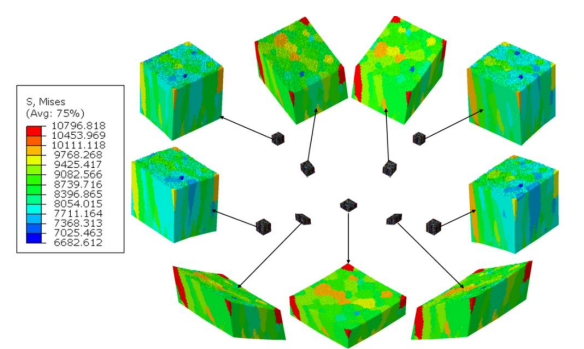
\includegraphics{Definitions/picture12.png}
  \label{fig:obraz12}
    \caption{Finite element mesh of the investigated TiN thin film columnar morphology.}
\end{figure}
 
\begin{figure}[H]
  \captionsetup{justification=centering}
  \centering
  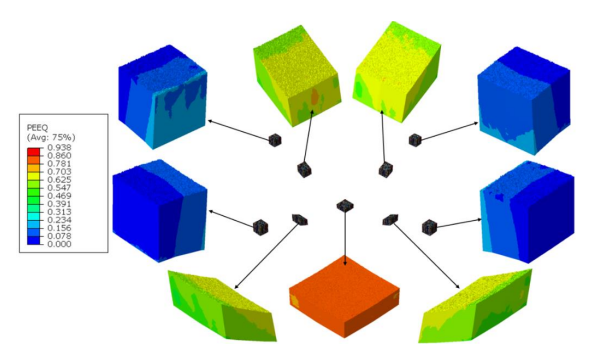
\includegraphics{Definitions/picture13.png}
  \label{fig:obraz13}
    \caption{Equivalent strain distribution in the DMR model after nanoindentation test.}
\end{figure}  
 
In the TiN film, especially between columns, large strain and stress irregularities can be observed at larger nanoindenter displacements. Prediction of these regions is important as stress and strain concentration zones can easily change into fracture initiation zones and lead to a destruction of the thin film that can be observed experimentally in Figure 14.
 
\begin{figure}[H]
  \captionsetup{justification=centering}
  \centering
  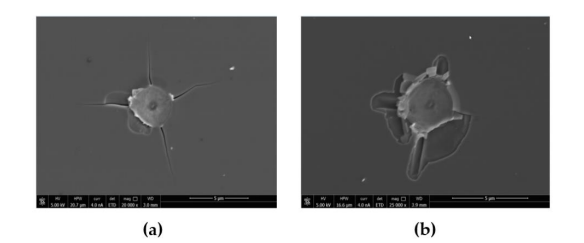
\includegraphics{Definitions/picture14.png}
  \label{fig:obraz14}
    \caption{SEM images revealing fractures in the \textbf{(a)} Si substrate and \textbf{(b)} TiN thin film after nanoindentation test.}
\end{figure}  
 
%%%%%%%%%%%%%%%%%%%%%%%%%%%%%%%%%%%%%%%%%%
\section{Discussion}
 
The V shape columnar TiN structure investigated within the work (Figure 8) is often reported in the literature when a low Si substrate temperature is considered [31–33]. As presented, such a columnar structure of a thin film can be quite heterogeneous. Therefore, precise control and understanding of a deposition operation are required to obtain desired thin film morphology. The developed kMC deposition model can serve as a support tool for such an investigation as it provides a reliable and explicit representation of columns. It can be used as a tool for the preliminary assessment of applied process parameters to evaluate their influence on the final thin film morphology. Additionally, such the digital model can be applied to more complex analysis of film behaviour under further processing conditions by means of the FE numerical simulations. Example of a numerical analysis of the TiN thin film from the mechanical properties point of view during the nanoindentation test was presented within the paper as a case study. Such numerical investigation can complement experimental investigations reported, e.g., in [34–36]. Since the column boundaries have been identified as the fracture initiation zones, the fracture resistance of the inter-column boundaries can be considered as the fracture resistance of the entire thin film. With the presented concept of combining the kMC deposition model and digital material representation finite element simulations it is possible to extend research in this area.
 
%%%%%%%%%%%%%%%%%%%%%%%%%%%%%%%%%%%%%%%%%%
\section{Conclusions}
 
\noindent Based on the presented results, it can be concluded that:
\begin{itemize}
\item	the kinetic Monte Carlo method is an adequate and feasible technique for numerical simulation of the PLD process and provides a reliable digital representation of microstructure morphology,
\item	the presented kMC PLD model can be adjusted to design the deposition processes of different nanolayered structures,
\item	the digital material representation model of the deposited thin films allows predicting inhomogeneities in stress/strain fields under deformation conditions,
\item   predicted local heterogeneities, especially in the interface area and along columns boundaries, can be further used to study fracture initiation and propagation. 
\end{itemize}
 
\funding{This research was supported by the National Science Centre (NCN–Poland) Research Project: No. 2015/17/D/ST8/01278.}
 
\acknowledgments{Numerical calculations have been performed with the use of the PLGrid Infrastructure.}
 
\conflictsofinterest{The author declares no conflict of interest.} 
 
\begin{adjustwidth}{-\extralength}{0cm}
\reftitle{References}
 
\begin{thebibliography}{999}
% Reference 1
\bibitem[Author1(year)]{ref-book1}
Greer, J. A. History and current status of commercial pulsed laser deposition equipment. \textit{J. Phys. D, Appl. Phys.} \textbf{2014}, \textit{47}, 1–10, doi:10.1088/0022-3727/47/3/034005.
% Reference 2
\bibitem[Author2(year)]{ref-book2}
Major, R.; Bonarski, J.; Morgiel, J.; Major, B.; Czarnowska, E.; Kustosz, R.; Lackner, J. M.; Waldhauser, W. Elastic TiN coating deposited on polyurethane by pulsed laser. \textit{Surface and Coatings Technology} \textbf{2006}, \textit{200}, 6340–6345, doi:10.1016/j.surfcoat.2005.11.003.
% Reference 3
\bibitem[Author3(year)]{ref-book3}
Kot, M.; Major, Ł.; Lackner, J. The tribological phenomena of a new type of TiN/a-C:H multilayer coatings. \textit{Mater. Des.} \textbf{2013}, \textit{51}, 280–286, doi:10.1016/j.matdes.2013.04.008.
% Reference 4
\bibitem[Author4(year)]{ref-book4}
Galinski, H.; Ryll, T.; Reibisch, P.; Schlagenhauf, L.; Schenker, I.; Gauckler, L. J. Temperature-dependent 2-D to 3-D growth transition of ultra-thin Pt films deposited by PLD. \textit{Acta Mater}. \textbf{2013}, \textit{61}, 3297–3303, doi:10.1016/j.actamat.2013.02.018.
% Reference 5
\bibitem[Author5(year)]{ref-book5}
Xu, X. H.; Zhang, R. Q.; Dong, X. Z.; Gehring, G. A. A study of the optimization of parameters for pulsed laser deposition using Monte Carlo simulation. \textit{Thin Solid Films} \textbf{2006}, 515, 2754–2759, doi:10.1016/j.tsf.2006.05.004.
% Reference 6
\bibitem[Author6(year)]{ref-book6}
Tekaya, A.; Ghulman, H. A.; Benameur, T.; Labdi, S. Cyclic Nanoindentation and Finite Element Analysis of Ti/TiN and CrN Nanocoatings on Zr-Based Metallic Glasses Mechanical Performance. \textit{J Mater Eng Perform} \textbf{2014}, \textit{23}, 4259–4270, doi:10.1007/s11665-014-1212-4.
% Reference 7
\bibitem[Author7(year)]{ref-book7}
Kopernik, M.; Milenin, A. Numerical modeling of substrate effect on determination of elastic and plastic properties of TiN nanocoating in nanoindentation test. \textit{Archives of Civil and Mechanical Engineering} \textbf{2014}, \textit{14}, 269–277, doi:10.1016/j.acme.2013.10.001.
% Reference 8
\bibitem[Author8(year)]{ref-book8}
Hajder, L.; Madej, Ł. Sphere packing algorithm for the generation of digital models of polycrystalline microstructures with heterogeneous grain sizes. \textit{Computer Methods in Materials Science} \textbf{2020}, \textit{20}, 22–30.
% Reference 9
\bibitem[Author9(year)]{ref-book9}
Perzynski, K.; Cios, G.; Szwachta, G.; Zych, D.; Setty, M.; Bala, P.; Madej, L. Numerical modelling of a compression test based on the 3D digital material representation of pulsed laser deposited TiN thin films. \textit{Thin Solid Films} \textbf{2019}, \textit{673}, 34–43, doi:10.1016/j.tsf.2019.01.012.
% Reference 10
\bibitem[Author10(year)]{ref-book10}
Feber, R. C.; Allen, L. D. F.; Grimmer, D. Monte carlo simulation of the nucleation of thin films. \textit{J. Vac. Sci. Technol.} \textbf{1971}, \textit{8}, 397–402, doi:10.1116/1.1314473.
% Reference 11
\bibitem[Author11(year)]{ref-book11}
Huang, H.; Gilmer, G. H.; Dı́az de la Rubia, T. An atomistic simulator for thin film deposition in three dimensions. \textit{J. Appl. Phys.} \textbf{1998}, \textit{84}, 3636–3649, doi:10.1063/1.368539.
% Reference 12
\bibitem[Author12(year)]{ref-book12}
Zhang, J.; Liu, C.; Shu, Y.; Fan, J. Growth and properties of Cu thin film deposited on Si(001) substrate: A molecular dynamics simulation study. \textit{Appl Surf Sci} \textbf{2012}, \textit{261}, 690–696, doi:10.1016/j.apsusc.2012.08.082.
% Reference 13
\bibitem[Author13(year)]{ref-book13}
Divi, S.; Chatterjee, A. Study of silicon thin film growth at high deposition rates using parallel replica molecular dynamics simulations. \textit{Energy Procedia} \textbf{2014}, \textit{54}, 270–280, doi:10.1016/j.egypro.2014.07.270.
% Reference 14
\bibitem[Author14(year)]{ref-book14}
Kosturek, R.; Malarz, K. New cellular automaton designed to simulate epitaxial films growth. \textit{Physica A: Statistical Mechanics and its Applications} \textbf{2005}, \textit{345}, 538–546, doi:10.1016/j.physa.2004.08.013.
% Reference 15
\bibitem[Author15(year)]{ref-book15}
Perzynski, K.; Major, L.; Madej, L.; Pietrzyk, M. Analysis of the stress concentration in the nanomultilayer coatings based on digital representation of the structure. \textit{Archives of Metallurgy and Materials} \textbf{2011}, \textit{56}, 393–399, doi:10.2478/v10172-011-0042-8.
% Reference 16
\bibitem[Author16(year)]{ref-book16}
El-Nashar, H. F.; Cerdeira, H. A. Random deposition-like model for two species in (2+1) dimensions. \textit{Surf Sci} \textbf{1998}, \textit{415}, 1–10, doi:10.1016/S0039-6028(98)00383-5.
% Reference 17
\bibitem[Author17(year)]{ref-book17}
Kim, D. H.; Kim, J. M. A model of random deposition with relaxation on fractal substrates. \textit{J. Stat. Mech.} \textbf{2010}, \textit{2010}, P08008, doi:10.1088/1742-5468/2010/08/P08008.
% Reference 18
\bibitem[Author18(year)]{ref-book18}
Kwak, W.; Kim, J. M. Random deposition model with surface relaxation in higher dimensions. \textit{Physica A: Statistical Mechanics and its Applications} \textbf{2019}, \textit{520}, 87–92, doi:10.1016/j.physa.2019.01.016.
% Reference 19
\bibitem[Author19(year)]{ref-book19}
Wei, W.; Cerdeira, H. A. Random-Like Deposition Model of Surface Growth Kinetics. \textit{Chinese Phys. Lett.} \textbf{1995}, \textit{12}, 755–758, doi:10.1088/0256-307X/12/12/014.
% Reference 20
\bibitem[Author20(year)]{ref-book20}
Ahn, J.-H.; Kwon, S.-H.; Kim, J.-H.; Kim, J.-Y.; Kang, S.-W. Theoretical Simulation of Surface Evolution Using the Random Deposition and Surface Relaxation for Metal Oxide Film in Atomic Layer Deposition' ' . \textit{J. Mater. Sci. Technol.} \textbf{2010}, \textit{24}, 371–374.
% Reference 21
\bibitem[Author21(year)]{ref-book21}
Landau, D. P.; Pal, S. Monte Carlo simulation of simple models for thin film growth by MBE. \textit{Thin Solid Films} \textbf{1996}, \textit{272}, 184–194, doi:10.1016/0040-6090(95)06945-3.
% Reference 22
\bibitem[Author22(year)]{ref-book22}
Goswami, J.; Ananthakrishna, G.; Shivashankar, S. A. Monte Carlo simulation of nucleation and growth of thin films. \textit{Bull. Mater. Sci.} \textbf{1997}, \textit{20}, 823–843, doi:10.1007/BF02747422.
% Reference 23
\bibitem[Author23(year)]{ref-book23}
Helin, W.; Zuli, L.; Kailun, Y. Monte Carlo simulation of thin-film growth on a surface with a triangular lattice. \textit{Vacuum} \textbf{1999}, \textit{52}, 435–440, doi:10.1016/S0042-207X(98)00328-5.
% Reference 24
\bibitem[Author24(year)]{ref-book24}
Mirabella, D. A.; Aldao, C. M. Surface growth by random deposition of rigid and wetting clusters. \textit{Surf Sci} \textbf{2016}, \textit{646}, 282–287, doi:10.1016/j.susc.2015.09.010.
% Reference 25
\bibitem[Author25(year)]{ref-book25}
Gall, D.; Kodambaka, S.; Wall, M. A.; Petrov, I.; Greene, J. E. Pathways of atomistic processes on TiN(001) and (111) surfaces during film growth: an ab initio study. \textit{J. Appl. Phys.} \textbf{2003}, \textit{93}, 9086, doi:10.1063/1.1567797.
% Reference 26
\bibitem[Author26(year)]{ref-book26}
Tholander, C.; Alling, B.; Tasnádi, F.; Greene, J. E.; Hultman, L. Effect of Al substitution on Ti, Al, and N adatom dynamics on TiN(001), (011), and (111) surfaces. \textit{Surf Sci} \textbf{2014}, \textit{630}, 28–40, doi:10.1016/j.susc.2014.06.010.
% Reference 27
\bibitem[Author27(year)]{ref-book27}
Sangiovanni, D. G.; Tasnádi, F.; Hultman, L.; Petrov, I.; Greene, J. E.; Chirita, V. N and Ti adatom dynamics on stoichiometric polar TiN(111) surfaces. \textit{Surf Sci} \textbf{2016}, \textit{649}, 72–79, doi:10.1016/j.susc.2016.01.031.
% Reference 28
\bibitem[Author28(year)]{ref-book28}
Perzynski, K.; Cios, G.; Szwachta, G.; Zych, D.; Setty, M.; Bala, P.; Madej, L. Evaluation of pulsed laser deposited thin films properties on the basis of the nanoindentation test. \textit{Procedia Engineering} \textbf{2017}, \textit{207}, 2191–2196, doi:10.1016/j.proeng.2017.10.980.
% Reference 29
\bibitem[Author29(year)]{ref-book29}
Fischer-Cripps, A. C. \textit{Nanoindentation}; Mechanical Engineering Series; Springer New York: New York, NY, 2011;
% Reference 30
\bibitem[Author30(year)]{ref-book30}
Madej, L.; Sieradzki, L.; Sitko, M.; Perzynski, K.; Radwanski, K.; Kuziak, R. Multi scale cellular automata and finite element based model for cold deformation and annealing of a ferritic–pearlitic microstructure. \textit{Comp. Mater. Sci.} \textbf{2013}, \textit{77}, 172–181, doi:10.1016/j.commatsci.2013.04.020.
% Reference 31
\bibitem[Author31(year)]{ref-book31}
Petrov, I.; Barna, P. B.; Hultman, L.; Greene, J. E. Microstructural evolution during film growth. \textit{J. Vac. Sci. Technol. A} \textbf{2003}, \textit{21}, S117–S128, doi:10.1116/1.1601610.
% Reference 32
\bibitem[Author32(year)]{ref-book32}
Cairney, J. M.; Harris, S. G.; Ma, L. W.; Munroe, P. R.; Doyle, E. D. Characterisation of TiN and TiAlN thin films deposited on ground surfaces using focused ion beam milling. \textit{J. Mater. Sci.} \textbf{2004}, \textit{39}, 3569–3575, doi:10.1023/B:JMSC.0000030708.70303.80.
% Reference 33
\bibitem[Author33(year)]{ref-book33}
Bhowmick, S.; Jayaram, V.; Biswas, S. Deconvolution of fracture properties of TiN films on steels from nanoindentation load-displacement curves. \textit{Acta Mater}. \textbf{2005}, \textit{53}, 2459–2467, doi:10.1016/j.actamat.2005.02.008.
% Reference 34
\bibitem[Author34(year)]{ref-book34}
Tilbrook, M. T.; Paton, D. J.; Xie, Z.; Hoffman, M. Microstructural effects on indentation failure mechanisms in TiN coatings: Finite element simulations. \textit{Acta Mater}. \textbf{2007}, \textit{55}, 2489–2501, doi:10.1016/j.actamat.2006.11.043.
% Reference 35
\bibitem[Author35(year)]{ref-book35}
Xie, Z. H.; Hoffman, M.; Munroe, P.; Bendavid, A.; Martin, P. J. Deformation mechanisms of TiN multilayer coatings alternated by ductile or stiff interlayers. \textit{Acta Mater}. \textbf{2008}, \textit{56}, 852–861, doi:10.1016/j.actamat.2007.10.047.
% Reference 36
\bibitem[Author36(year)]{ref-book36}
Peng, S.; Xu, J.; Munroe, P.; Xie, Z. Sandwich-structured, damage-resistant TiN/graded TiSiN/TiSiN film. \textit{Results in Physics} \textbf{2019}, 12, 543–554, doi:10.1016/j.rinp.2018.12.019.
\end{thebibliography}
 
\end{adjustwidth}
\end{document}

